%% KSE 2026 -- Fusion of Embodied AI and Soft Robotics
%% Differentiable Neural-Operator Surrogate for Vision-Based Tactile Sensing and Control
%% Compile on Overleaf (IEEEtran is built in) or locally with:
%%   pdflatex main && bibtex main && pdflatex main && pdflatex main
\documentclass[conference]{IEEEtran}
\IEEEoverridecommandlockouts

\usepackage{cite}
\usepackage{amsmath,amssymb,amsfonts}
\usepackage{graphicx}
\usepackage{booktabs}
\usepackage{xcolor}
\usepackage{url}
\usepackage{tikz}
\usetikzlibrary{arrows.meta,positioning,fit,backgrounds}
\usepackage[hidelinks]{hyperref}

\newcommand{\relL}{\mathrm{rel}\text{-}L_2}
\newcommand{\todo}[1]{\textcolor{red}{[TODO: #1]}}
\setlength{\emergencystretch}{3em} % absorb minor overfull lines in narrow IEEE columns

%% ---------------------------------------------------------------------------
%% RESULT NUMBERS -- SINGLE SOURCE OF TRUTH
%% Every result number in the body and the tables is emitted from this block.
%% When the v2 ground truth lands, edit ONLY this block; the prose is written to
%% survive the substitution (no hard-coded magnitudes such as "an order of
%% magnitude" that a shifted number could falsify).
%% GT PROVENANCE OF THE VALUES BELOW: pre-v2 (gel_nz=4, d_hat=1e-4, tol 3e-4).
%% ---------------------------------------------------------------------------
% -- RQ1 bake-off: field error (rel-L2), direction error (deg), advantage vs LR-FNO
\newcommand{\lrfnoErr}{0.060}       \newcommand{\lrfnoDir}{1.5}
\newcommand{\fnoErr}{0.074}         \newcommand{\fnoDir}{1.6}   \newcommand{\fnoAdv}{1.23}
\newcommand{\unetErr}{0.085}        \newcommand{\unetDir}{2.2}  \newcommand{\unetAdv}{1.42}
\newcommand{\deeponetErr}{0.115}    \newcommand{\deeponetDir}{3.2} \newcommand{\deeponetAdv}{1.91}
\newcommand{\galerkinErr}{0.151}    \newcommand{\galerkinDir}{4.1} \newcommand{\galerkinAdv}{2.52}
\newcommand{\tactoErr}{0.656}       \newcommand{\tactoDir}{69.6} \newcommand{\tactoAdv}{10.90}
\newcommand{\cmErr}{0.693}          \newcommand{\cmDir}{26.0}   \newcommand{\cmAdv}{11.51}
\newcommand{\hertzErr}{0.672}       \newcommand{\hertzDir}{26.0} \newcommand{\hertzAdv}{11.17}
\newcommand{\taximErr}{0.302}       \newcommand{\taximDir}{9.3} \newcommand{\taximAdv}{5.01}
\newcommand{\mlpErr}{0.545}         \newcommand{\mlpDir}{41.9}  \newcommand{\mlpAdv}{9.06}
% span of the advantage over the classical/analytic baselines (min--max of *Adv above)
\newcommand{\baselineSpanLo}{5.0}   \newcommand{\baselineSpanHi}{11.5}
% -- RQ1 per-regime error and slip heads
\newcommand{\errNormal}{0.046}  \newcommand{\errStick}{0.052}
\newcommand{\errPartial}{0.061} \newcommand{\errFull}{0.086}
\newcommand{\slipMacroF}{0.931} \newcommand{\slipBinF}{0.969}
% -- RQ1 five-seed table and the local-refinement ablation
\newcommand{\lrfnoMean}{0.0590} \newcommand{\lrfnoStd}{0.0014} \newcommand{\lrfnoT}{4.72}
\newcommand{\fnoMean}{0.0780}   \newcommand{\fnoStd}{0.0081}
\newcommand{\unetMean}{0.0890}  \newcommand{\unetStd}{0.0067}  \newcommand{\unetT}{-2.16}
\newcommand{\ufnoMean}{0.0634}  \newcommand{\ufnoStd}{0.0113}  \newcommand{\ufnoT}{1.85}
\newcommand{\refineGain}{24}    % LR-FNO improvement over the trunk, percent
\newcommand{\seedStableX}{6}    % LR-FNO seed-stability factor vs the trunk
\newcommand{\unetSigmaGap}{4}   % LR-FNO-to-U-Net gap in std devs
% -- RQ2 parametric extrapolation (LR-FNO, then plain trunk)
\newcommand{\oodR}{2.10} \newcommand{\oodMu}{1.63} \newcommand{\oodE}{1.32}
\newcommand{\oodRtrunk}{2.60} \newcommand{\oodMutrunk}{1.95} \newcommand{\oodEtrunk}{1.36}
% -- RQ3 speed
\newcommand{\opFps}{5600} \newcommand{\opLatency}{0.18}
\newcommand{\ipcFps}{0.192} \newcommand{\speedup}{29{,}182}
% -- RQ4 differentiable control
\newcommand{\agLoss}{1.94\times10^{-10}} \newcommand{\esLoss}{2.19\times10^{-10}}
\newcommand{\oracleLoss}{8.06\times10^{-12}}
\newcommand{\agQueries}{300} \newcommand{\esQueries}{19{,}200} \newcommand{\budgetX}{64}
\newcommand{\agWall}{18.24} \newcommand{\esWall}{438.02} \newcommand{\wallX}{24}
\newcommand{\agHit}{81} \newcommand{\esHit}{5824} \newcommand{\hitX}{72}
% -- RQ5 sensor / image-space inversion
\newcommand{\flowCos}{0.998}
\newcommand{\trackStick}{0.14} \newcommand{\trackPartial}{0.26} \newcommand{\trackFull}{0.39}
\newcommand{\invMag}{11.8} \newcommand{\invDir}{4.8} \newcommand{\invDirWorst}{1.1}
\newcommand{\rewardClosed}{99.8} \newcommand{\fdErr}{4.96}

\begin{document}

\title{A Differentiable Neural-Operator Surrogate for\\
Vision-Based Tactile Sensing and Control}

\author{\IEEEauthorblockN{Anonymous Authors}}

\maketitle

\begin{abstract}
Vision-based tactile sensors (VBTS) such as GelSight and DIGIT let robots perceive
contact through the deformation of a soft, marker-printed gel. Simulating them
faithfully requires solving frictional elastic contact, which is expensive,
non-differentiable, and ill-suited to closed-loop control. We learn a
locally refined \emph{Fourier neural operator} (LR-FNO) that maps a contact
field to the surface marker-displacement field---an adaptation of the U-FNO
family with a lightweight local refinement head---and use it as a
differentiable,
solver-faithful, hardware-light surrogate for the contact solver. Trained on and
benchmarked against finite-element IPC/GIPC frictional-contact physics generated
with libuipc in a TacEx-style setup, the surrogate yields three results.
(i)~\emph{Field-to-field framing
is the key}: because surface displacement is a \emph{non-local} (Green's-function)
response, an operator that learns global spectral convolutions beats a local
per-point MLP by $\mlpAdv\times$ and the analytic and learned VBTS baselines by
$\baselineSpanLo$--$\baselineSpanHi\times$ on the same IPC ground truth; adding
local refinement to the spectral trunk improves it by a further $\refineGain\%$,
consistently across five seeds. Because every model is fit on the same targets,
this ranking is a property of the architectures, not of the ground truth: we
verify it by re-deriving the ground truth at a $5\times$ finer discretisation and
showing the ranking and the margins are unchanged.
(ii)~\emph{Differentiability buys
sample-efficient control}: learning a goal-conditioned policy by backpropagation
through the frozen operator reaches the target with $\hitX\times$ fewer model
queries, runs $\wallX\times$ faster, and reaches lower final loss than a
gradient-free baseline. (iii)~\emph{The sensor pipeline is autograd-connected}: a
torch marker-dot renderer composes with the operator so that applied shear can be
optimized from the rendered tactile image alone. We close with an honest account
of scope: the surrogate is faithful to the \emph{solver}, whose own residual
discretisation error we measure and report rather than assume away; it does not
model real sensor noise; the environment is single-step and quasi-static; and the
present geometry is sphere-centric.
\end{abstract}

\begin{IEEEkeywords}
vision-based tactile sensing, neural operator, differentiable simulation,
soft robotics, embodied AI, contact mechanics
\end{IEEEkeywords}

\section{Introduction}\label{sec:intro}

Vision-based tactile sensors (VBTS)---GelSight~\cite{yuan2017gelsight},
DIGIT~\cite{lambeta2020digit}, and marker-gel variants---give robots a dense,
high-resolution sense of touch by imaging the deformation of a soft elastomer
printed with a grid of markers. They have become a workhorse of contact-rich
manipulation, but \emph{simulating} them is hard for a structural, not incidental,
reason: the signal a VBTS reports is the \emph{solution} of a frictional,
hyper-elastic contact problem. This forces existing simulators onto one horn of a
trilemma, and each horn is a concrete bottleneck.
\emph{(B1)~Fidelity vs.\ speed.} High-fidelity finite-element (FEM/IPC) solvers
reproduce the physics but cost seconds per frame---too slow to sit inside a
control or reinforcement-learning loop. The fast phenomenological simulators buy
that speed by discarding physics: TACTO~\cite{wang2022tacto} renders gel
deformation kinematically \emph{without friction}, while
Taxim~\cite{si2022taxim} and FOTS~\cite{zhao2023fots} use example-based
\emph{linear superposition}. Both are first-order and break down exactly in the
stick--partial-slip--slip regime that manipulation depends on.
\emph{(B2)~Fidelity with differentiability, but at engine cost.} A recent line of
differentiable physics-based tactile engines---DiffTactile~\cite{si2024difftactile}
and GPU contact solvers such as TacIPC and Taccel~\cite{taccel2025}---restores both
fidelity and gradients, but pays by running a full contact solve \emph{every step}
and inherits a known pathology: gradients taken through stiff, near-discontinuous
contact can be \emph{worse} than gradient-free estimates~\cite{suh2022diffsim}.
\emph{(B3)~Representation.} Learned tactile models are typically posed as
per-point or image regressors, implicitly assuming a \emph{local} contact
response---yet the surface displacement of a bonded gel is a \emph{non-local}
(Green's-function) field, so the locality assumption is a modelling error, not a
detail. No existing tool is simultaneously FEM-fidelity in slip, cheaply and
cleanly differentiable, and millisecond-latency.

We take a different route. Rather than approximate the renderer, we learn the
\emph{operator} that the FEM solver computes: a map from a compact description of
the contact (indentation profile and tangential drive) to the full surface
marker-displacement field. We instantiate it as a locally refined Fourier
neural operator (LR-FNO) and treat it as a drop-in surrogate for the solver that is
(a)~\emph{solver-faithful}---validated frame-by-frame against IPC/GIPC
frictional-contact ground truth, which we take to mean fidelity to the FEM solver
and not to a physical sensor, a distinction we keep throughout;
(b)~\emph{differentiable}, so gradients flow
through it by autograd;
and (c)~\emph{hardware-light and mesh-free}, running on a single consumer GPU.
The move dissolves the trilemma by relocating the physics cost \emph{offline}: an
IPC solver pays once to generate ground truth (B1), and the smooth learned map
replaces the per-step solve with a millisecond forward pass whose gradients are
clean (B2). The remaining question is whether a \emph{generic} operator suffices;
we show it does not, and that the non-local field$\to$field framing (B3) is what
makes it work.

This positions our work squarely at the fusion of embodied AI and soft robotics:
a fast, differentiable model of a soft tactile sensor that can sit inside a
control loop. Our contributions are:

\begin{enumerate}
\item \textbf{A physics-matched tactile operator architecture, LR-FNO (attacks B3, B1).}
We build the surrogate so that each architectural element mirrors a mechanism of
the contact physics it replaces. A global spectral trunk supplies the non-local,
Green's-function support that bonded-gel elasticity demands---posing the problem
as \emph{field$\to$field} rather than per-point regression---and a lightweight
local-refinement path ($+3.3\%$ parameters) restores the sharp near-contact-edge
features that frictional slip creates and a band-limited spectral basis smooths
away. Both design choices are validated separately on the \emph{same} IPC ground
truth: the non-local trunk beats an otherwise-matched local per-point MLP by
$\mlpAdv\times$ and reimplemented TACTO-, Taxim/FOTS-, and Cattaneo--Mindlin-style
baselines by $\baselineSpanLo$--$\baselineSpanHi\times$; the refinement path
improves the trunk by a further $\refineGain\%$ on every one of five seeds
(paired $t{=}\lrfnoT$) (Sec.~\ref{sec:exp-accuracy}).
\item \textbf{Physical information enters the network as fields, not parameters.}
The operator consumes contact state in physical form: a geometric
penetration-depth field and a friction-drive field masked to the contact
footprint, sampled on the marker grid, with material scalars $(\mu,E)$ as
conditioning and a Coulomb-consistent contact-mode taxonomy supervising an
auxiliary multitask head. This encoding is what lets a single frozen model span
normal, stick, partial-slip, and full-slip contact, and degrade gracefully
(at most $\oodR\times$) rather than fail under out-of-range indenter radius and
material parameters (Sec.~\ref{sec:exp-accuracy}).
\item \textbf{Differentiable control through a frozen operator (attacks B2).}
Backpropagating a goal-conditioned policy through the frozen surrogate reaches a
tactile target with $\hitX\times$ fewer target-reaching model queries and
$\wallX\times$ less wall-clock than evolution strategies, while also reaching lower
final loss (Sec.~\ref{sec:exp-control}). We find the often-reported pathology of
differentiable simulators~\cite{suh2022diffsim} does \emph{not} bite here, and
explain why.
\item \textbf{An autograd-connected sensor pipeline (extends B2 to the image).}
A torch marker-dot renderer composes with the operator, $\mathrm{render}\circ
\mathrm{LR\mbox{-}FNO}$, so a control action can be recovered from the rendered tactile
\emph{image} by gradient descent (Sec.~\ref{sec:exp-sensor}).
\item \textbf{A ground-truth error budget---and evidence the conclusions do not
rest on it.} Learned tactile models are routinely trained on simulated contact
whose own discretisation error is never reported. We audit ours instead. The audit
yields a reusable finding: in barrier-based (IPC) contact the barrier width
$\hat d$ and the indenter's facet resolution are \emph{one} knob, not two---refining
either alone produces spurious non-monotone convergence---and once they are refined
together the field contracts at first order (Appendix~\ref{app:conv}). We then do
the thing the number cannot do on its own: re-derive the ground truth at a
$5\times$ finer discretisation, retrain every model on it, and show that the
architecture ranking and margins are unchanged (Sec.~\ref{sec:exp-gtinvariance}).
The comparison is therefore a statement about the architectures, not about the
solver settings.
\end{enumerate}
Throughout, we keep an honest scope: the surrogate is faithful to a \emph{solver},
not to a physical sensor; we report the solver's residual error rather than assume
it away, and we delimit the current environment and geometry
(Sec.~\ref{sec:limits}).

\section{Related Work}\label{sec:related}

\textbf{Fast phenomenological VBTS simulators.}
The first generation of tactile simulators optimises for rendering speed.
TACTO~\cite{wang2022tacto} drives a depth-based renderer from a rigid-body engine
and produces gel images kinematically, with \emph{no} frictional contact model;
Taxim~\cite{si2022taxim} and FOTS~\cite{zhao2023fots} calibrate example-based
\emph{linear-superposition} maps from contact geometry to the optical and
marker-motion signal. \emph{What they achieve:} real-time, easy-to-calibrate
optical simulation adequate for perception pretraining. \emph{Their bottleneck (B1):}
the contact response is modelled only to first order, so tangential marker motion
in the stick--partial-slip--slip transition---the very signal used for grasp
stability and slip detection---is not physical. We keep their spirit of a fast
forward model but ground it frame-by-frame in full frictional-contact physics rather
than in a linear or kinematic proxy, and we quantify the gap: on identical IPC
ground truth our operator improves on reimplemented TACTO-, Taxim/FOTS-, and
analytic Cattaneo--Mindlin-style baselines by $5.0$--$11.5\times$
(Sec.~\ref{sec:exp-accuracy}).

\textbf{Differentiable, physics-based tactile simulation.}
A second generation restores physical fidelity \emph{and} gradients.
DiffTactile~\cite{si2024difftactile} exposes an end-to-end differentiable
soft-contact pipeline, and GPU incremental-potential solvers such as TacIPC and
Taccel~\cite{taccel2025}, building on GIPC-style barrier
contact~\cite{huang2024gipc,nguyen2024tacex}, deliver penetration-free frictional
contact at interactive rates. \emph{What they achieve:} contact whose numerical
error is controlled by explicit parameters, with usable sensitivities. \emph{Their bottleneck (B2):} fidelity is paid for by executing a
full contact solve at \emph{every} simulation step, and differentiating through
stiff barrier/near-discontinuous contact is exactly the regime where analytic
gradients can degrade~\cite{suh2022diffsim}. Our position is deliberately
complementary rather than competitive: we \emph{use} such a solver (libuipc/GIPC)
as the ground-truth generator, then \emph{amortise} it into a single frozen
operator whose forward pass is milliseconds and whose gradient is smooth by
construction. We solve the amortisation-and-gradient bottleneck, not the online
solver bottleneck.

\textbf{Neural operators as PDE surrogates.}
FNO~\cite{li2021fno} and DeepONet~\cite{lu2021deeponet} learn maps between function
spaces and are now standard surrogates for PDE solution
operators~\cite{kovachki2023neuraloperator}; attention-based variants such as the
Galerkin Transformer~\cite{cao2021galerkin} and global--local hybrids such as
U-FNO~\cite{wen2022ufno}, which augment Fourier layers with a local convolutional
path, extend the family. \emph{What this line achieves:} mesh-free, resolution-flexible
operators for canonical parametric PDEs. \emph{The gap (B3):} these operators are
almost never applied to frictional \emph{contact}, and learned \emph{tactile}
models instead default to per-point or per-pixel regression, silently assuming a
local response. We argue this is the wrong inductive bias for a bonded gel, whose
surface displacement is a non-local Green's-function field, and we make the case
empirically: the field$\to$field spectral operator beats an otherwise-matched
local MLP by $9.1\times$ on the same data, and a lightweight local-refinement head
(adapting the U-FNO global--local idea to near-contact sharp features) adds a
further $24\%$ across five seeds. We thus bring operator learning to tactile
contact and exploit its \emph{non-locality} and \emph{differentiability}, not only
its accuracy.

\textbf{Differentiable simulation for control.}
Differentiable physics~\cite{hu2020difftaichi} promises low-variance policy
gradients, but Suh~\textit{et al.}~\cite{suh2022diffsim} show that stiff or
discontinuous dynamics can make these gradients \emph{worse} than zeroth-order
estimates---the pathology underlying B2. Rather than assume it away, we test it
directly by backpropagating a policy through the learned contact operator, and
find the gradients are clean for the present one-step quasi-static problem: policy
learning reaches the target with $72\times$ fewer model queries and $24\times$
less wall-clock than a gradient-free baseline (Sec.~\ref{sec:exp-control}). The
learned smooth surrogate is precisely what removes the stiffness that makes B2
bite.

\smallskip\noindent\textbf{Positioning.} Table~\ref{tab:pipelines} places these
pipelines side by side on the capabilities that matter for in-the-loop tactile
control. The comparison is qualitative by design: each entry reflects a system's
construction rather than a head-to-head benchmark, since cross-paper numbers
target different sensor outputs and are not comparable (Sec.~\ref{sec:exp-accuracy}
instead re-implements the marker cores on identical ground truth). Read this way,
the fast phenomenological simulators match us on latency and amortisation but
discard the slip physics; the differentiable physics engines match us on fidelity
and gradients but pay a full contact solve every step; and our surrogate is the
only row that is at once slip-faithful, cheaply and \emph{smoothly}
differentiable, free of an online solve, and millisecond-latency---the trade being
the geometric generality the physics-based engines retain and we approach only by
few-shot adaptation (Sec.~\ref{sec:exp-gen}).

\begin{table}[t]
\centering
\caption{Where the learned surrogate sits among tactile-simulation pipelines.
Entries reflect each system's design, not a head-to-head benchmark.
``Amort.''\ = no online contact solve; ``Lat.''\ is per single frame
(``solve'' = a full per-step contact solve); ``Geom.''\ is the object scope
(``sph.+FT'' = sphere-trained plus few-shot adaptation). Modern batched GPU
engines can raise aggregate throughput, but not single-frame latency or gradient
smoothness (Sec.~\ref{sec:exp-speed}).}
\label{tab:pipelines}
\setlength{\tabcolsep}{3.5pt}
\scriptsize
\begin{tabular}{@{}llcccl@{}}
\toprule
Method & Contact model & Diff. & Amort. & Lat. & Geom. \\
\midrule
TACTO~\cite{wang2022tacto} & kinematic & $\times$ & \checkmark & ms & any \\
Taxim/FOTS~\cite{si2022taxim,zhao2023fots} & linear & $\times$ & \checkmark & ms & any \\
DiffTactile~\cite{si2024difftactile} & soft FEM & \checkmark & $\times$ & solve & any \\
TacIPC/Taccel~\cite{taccel2025} & IPC (barrier) & \checkmark & $\times$ & solve & any \\
\textbf{LR-FNO (ours)} & \textbf{FEM-fid.} & \checkmark & \checkmark & \textbf{0.18\,ms} & sph.+FT \\
\bottomrule
\end{tabular}
\end{table}

\section{Problem Formulation and Ground Truth}\label{sec:setup}

\textbf{Three model tiers.} We deliberately separate roles
(Table is implicit): a \emph{high-fidelity but slow ground truth} (IPC/GIPC FEM) generates
data and is the yardstick; an \emph{analytic validator}
(Hertz~\cite{johnson1985contact} + Cattaneo--Mindlin~\cite{mindlin1949}) checks the
ground truth and provides a first-principles baseline; and the \emph{fast
differentiable surrogate} (LR-FNO) is our contribution.

\textbf{FEM ground truth.} We simulate a representative thin-gel
$20\times20\times3$\,mm tactile sensor with
IPC/GIPC frictional contact using libuipc in a TacEx-style
setup~\cite{huang2024gipc,nguyen2024tacex}. We selected IPC because its barrier
contact exposes the numerical parameters that govern the tangential channel
\emph{explicitly} --- the barrier activation distance $\hat d$, the indenter's
surface discretisation, the gel mesh, and the time step --- so the ground-truth
error can be \emph{measured and reduced} rather than assumed. The penalty-based
deformable contact we first used (PhysX) offers no such handle and proved severely
mesh-dependent in exactly the channel this paper is about: refining the gel mesh
changed the \emph{tangential} displacement field by $84\%$ relative $L_2$
($24\!\to\!32$). This is a ground-truth engineering choice, not a claim of our own
about IPC's convergence order; we make no assertion that IPC yields
\emph{mesh-consistent} friction, and we quantify our own residual error below.

\textbf{Ground-truth convergence and residual error.} We report a convergence study
of the ground truth itself (Appendix~\ref{app:conv}). Three numerical axes control
the tangential field and must be refined \emph{jointly}. Critically, $\hat d$ is
coupled to the indenter's facet resolution: the barrier cannot resolve a sphere
whose own discretisation error (the facet sagitta $\approx e^2/8R$) exceeds
$\hat d$, so refining either alone yields spurious non-monotone convergence curves.
Holding $\hat d/\text{sagitta}\approx 7.5$, the field contracts at first order along
the refinement path (successive differences $33.5\%\!\to\!6.9\%$, ratio
$\approx 0.25$, on all three contact modes). Our production configuration
(gel $32\times32\times24$, indenter subdivision $4$, $\hat d=2.5\times10^{-5}$\,m,
$\Delta t=5$\,ms, Newton tolerance $10^{-5}$) refines every axis jointly. We do
\emph{not} claim a converged ground truth: the gel-mesh axis contracts slowly, and
we estimate the residual from the observed convergence order and the last
refinement step rather than against any single ``fine'' run, since no affordable
run is exact (Appendix~\ref{app:conv}). Instead of arguing that the residual is
negligible, we bound its \emph{consequence} empirically in
Sec.~\ref{sec:exp-gtinvariance}. At this tolerance the solver is deterministic
(run-to-run spread $0.03$--$0.32\%$), so no replicate averaging is used.
A spherical indenter
($R\in[2,6]$\,mm) indents the bonded thin gel by $0.15$--$0.75$\,mm and shears it
through the stick--partial-slip--full-slip regimes.
Each frame exports the surface displacement field
$\mathbf{u}\in\mathbb{R}^{M\times3}$ sampled on a $32\times32$ marker grid. The
analytic Hertz/Cattaneo--Mindlin model is used only as a first-principles
baseline: the finite, substrate-confined gel is expected to deviate from the
half-space solution, which is precisely why IPC/GIPC is the ground truth. We sweep
indenter radius $R$, friction $\mu$, and gel stiffness $E$ to produce a
structured-tetrahedron, resolution-24 benchmark of $N{=}2520$ frames ($2120$
train / $400$ deterministic stratified test). A normal-contact top-up keeps all
regimes represented, yielding normal / stick / partial-slip / full-slip counts of
$425/712/895/488$ (test: $68/113/142/77$). The gel bottom is bonded as a pinned
Dirichlet boundary to a rigid transparent support; the top is the contact
surface, the sides are free, and the indenter is rigid and displacement-controlled.
Each element of this boundary setup is chosen to match the physical sensor
rather than for numerical convenience. \emph{Bottom (pinned Dirichlet).} In a
real VBTS the elastomer is cast or glued directly onto the rigid, transparent
camera window (acrylic or glass), so zero displacement at the base is the
physically correct condition, not an idealisation. It is also what defines the
mechanical regime: a bonded, few-millimetre gel responds as a
substrate-confined \emph{thin layer}, whose displacement field differs
systematically from the unbounded half-space assumed by Hertz-type analytic
models---one of the reasons an FEM/IPC ground truth is needed at all. Finally,
the rigid anchor is what keeps the tangential channel well-posed: with a
compliant bottom constraint the sheared gel translates near-rigidly, and this
common-mode drift dominates the \emph{relative} marker motion that carries the
stick--slip signal; pinning the base removes the drift mode by construction.
\emph{Sides (traction-free).} The contact radius stays small compared to the
lateral half-width of the pad even at the deepest indentation, so the side
walls carry negligible load; leaving them free avoids imposing an artificial
lateral stiffness that a clamped side wall would add. \emph{Indenter (rigid,
displacement-controlled).} The indenting object is orders of magnitude stiffer
than the gel ($E\!\sim\!10^{5}$\,Pa), so its own deformation is negligible, and
displacement control (prescribed depth, then prescribed tangential travel)
yields a deterministic loading path through the stick--partial-slip--full-slip
sequence, whereas force control would make the regime labels depend on the
solver's friction state. \emph{Top (frictional contact).} The top face is left
free except for the IPC barrier contact itself, which enforces
non-penetration and Coulomb friction without a user-tuned penalty stiffness;
its numerical error is instead governed by the explicit barrier distance
$\hat d$, which we refine (Appendix~\ref{app:conv}).
At the Newton tolerance we use ($10^{-5}$) repeated solves agree to
$0.03$--$0.32\%$, so each frame is a single solve ($K{=}1$) and no replicate
averaging is required.
\iffalse
Because GPU IPC solves are not bitwise repeatable, each frame's target is a
robust average over up to $K{=}5$ repeated solves: an adaptive filter keeps the
largest replicate subset (two to five) whose mean pairwise tangential distance
stays below a fixed tolerance.
\fi

\textbf{Contact-mode taxonomy.} Each frame is labelled
normal / stick / partial-slip / full-slip by tangential-drive thresholds; we
use these labels both as a multitask target and for per-regime error reporting.

\begin{figure*}[t]
\centering
\resizebox{0.96\textwidth}{!}{%
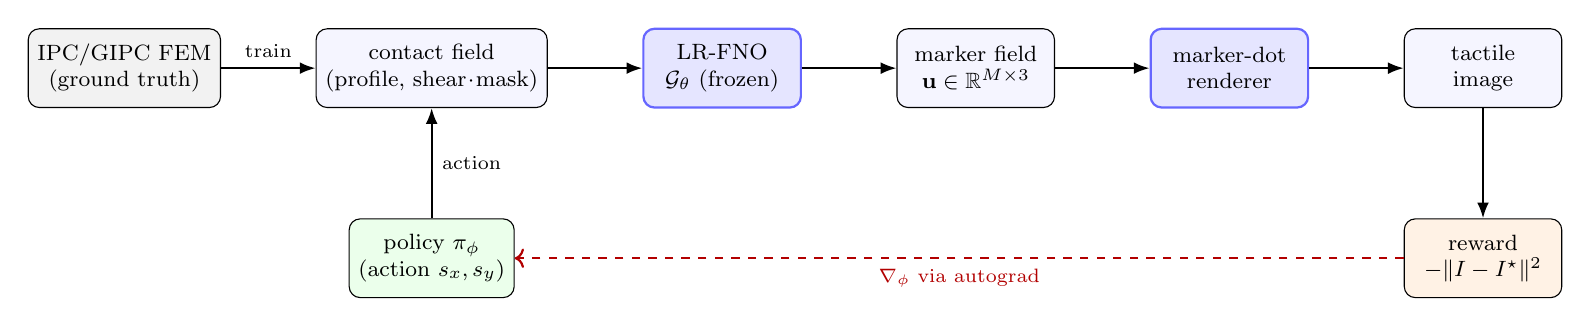
\begin{tikzpicture}[
  node distance=7mm and 12mm,
  box/.style={draw, rounded corners, align=center, minimum height=10mm,
    minimum width=20mm, font=\footnotesize, fill=blue!4},
  gt/.style={box, fill=gray!10},
  ours/.style={box, fill=blue!10, draw=blue!60, thick},
  grad/.style={->, red!70!black, dashed, thick},
  flow/.style={-{Latex[length=2mm]}, thick}]

  \node[gt] (fem) {IPC/GIPC FEM\\(ground truth)};
  \node[box, right=of fem] (ctx) {contact field\\$(\text{profile},\,\text{shear}\!\cdot\!\text{mask})$};
  \node[ours, right=of ctx] (fno) {LR-FNO\\$\mathcal{G}_\theta$ (frozen)};
  \node[box, right=of fno] (disp) {marker field\\$\mathbf{u}\in\mathbb{R}^{M\times3}$};
  \node[ours, right=of disp] (rend) {marker-dot\\renderer};
  \node[box, right=of rend] (img) {tactile\\image};

  \node[box, below=14mm of ctx, fill=green!8] (pol) {policy $\pi_\phi$\\(action $s_x,s_y$)};
  \node[box, below=14mm of img, fill=orange!10] (rew) {reward\\$-\lVert I-I^\star\rVert^2$};

  \draw[flow] (fem) -- node[above,font=\scriptsize]{train} (ctx);
  \draw[flow] (ctx) -- (fno);
  \draw[flow] (fno) -- (disp);
  \draw[flow] (disp) -- (rend);
  \draw[flow] (rend) -- (img);
  \draw[flow] (pol.north) -- node[right,font=\scriptsize]{action} (ctx.south);
  \draw[flow] (img) -- (rew);
  \draw[grad] (rew.west) -- node[below,font=\scriptsize]{$\nabla_\phi$ via autograd} (pol.east);
\end{tikzpicture}
}
\caption{The differentiable tactile pipeline. The LR-FNO surrogate is trained once
against FEM ground truth, then frozen. A marker-dot renderer turns its output
field into a tactile image. The policy is trained by backpropagating an image- or
field-space reward through the frozen surrogate (red, dashed).}
\label{fig:pipeline}
\end{figure*}

\section{Method}\label{sec:method}

\subsection{Neural-operator preliminaries}\label{sec:method-no}
A conventional network learns a map between finite-dimensional vectors; a
\emph{neural operator} learns a map $\mathcal{G}:\mathcal{A}\to\mathcal{U}$
between \emph{function spaces} from pairs of input--output
functions~\cite{kovachki2023neuraloperator}. In our problem the input function
$a\in\mathcal{A}$ is the contact field on the gel surface---an indentation-depth
profile stacked with a tangential-drive channel masked to the contact
footprint---and the output function $u\in\mathcal{U}$ is the surface
marker-displacement field; the $32\times32$ marker grid is merely the
discretization on which both happen to be observed, not the object being
learned. A neural operator composes layers of the form
\begin{equation}
v_{t+1}(x) = \sigma\!\Big(W\,v_t(x) + (\mathcal{K}v_t)(x)\Big),
\label{eq:no-layer}
\end{equation}
i.e.\ a pointwise linear term plus a learned \emph{kernel integral operator}
$(\mathcal{K}v)(x)=\int_{D}\kappa_\theta(x,y)\,v(y)\,dy$,
so every layer has global support by construction. This abstraction is not
merely convenient here---it is the form the physics already takes. For a bonded
elastic layer the surface response to a contact traction $t$ is exactly a
kernel integral, $u(x)=\int G(x,y)\,t(y)\,dy$, with $G$ the Green's function of
the substrate-confined gel; friction and finite deformation make the true map
nonlinear, but they do not remove its non-local structure. Learning
$\mathcal{G}$ therefore amounts to learning a (nonlinear) Green's operator for
the sensor.

\subsection{The FNO trunk}\label{sec:method-fno}
The cost of Eq.~\eqref{eq:no-layer} is the integral. The Fourier neural
operator (FNO)~\cite{li2021fno} makes it tractable by restricting the kernel to
be translation-invariant, $\kappa_\theta(x,y)=\kappa_\theta(x-y)$, so the
integral becomes a convolution and, by the convolution theorem, a
multiplication in the Fourier domain:
\begin{equation}
(\mathcal{K}v)(x) = \mathcal{F}^{-1}\!\big(R_\theta \cdot \mathcal{F}v\big)(x),
\end{equation}
where $R_\theta$ parameterizes the kernel directly by its lowest $k$ Fourier
modes and the FFT gives quasi-linear cost. Two properties follow. First, the
\emph{global receptive field in every layer} matches the Green's-function
physics above: indenting one point moves a whole neighbourhood, and a spectral
kernel propagates that influence across the pad in a single layer. This is the
crux empirically, not just conceptually: a \emph{local} map (a per-point MLP
fed the full parameter vector) can fit the easy param$\to$field direction but
\emph{collapses} on field$\to$field ($\relL=0.545$, $42^\circ$ direction
error), whereas the FNO holds. The operator framing is therefore not a
modelling convenience but the source of the result. Second, however, the
truncation to $k$ modes makes each spectral layer \emph{band-limited}: it
represents smooth, long-wavelength structure cheaply but systematically blurs
sharp, localized features.

\subsection{From FNO to LR-FNO: restoring the local physics}
\label{sec:method-lrfno}
That band limit is not an abstract concern in tactile contact---the most
informative part of the field lives exactly where it bites. The stick--slip
transition creates a sharp annulus at the contact edge, and the penetration
profile itself has a kink at the contact boundary; both sit in the high-order
modes a truncated spectral basis smooths away, while the translation-invariance
assumption is itself only approximate for a finite bonded pad. Our main model,
\emph{LR-FNO}, therefore augments the spectral trunk with a lightweight local
path: a two-layer convolutional stem added to the lifting layer, and a small
refinement head that reads the trunk output, the local features, and the raw
input. The division of labour mirrors the physics: the spectral trunk carries
the smooth, non-local Green's response, while the convolutional path---whose
small kernels are exactly the high-frequency, spatially-local complement of the
truncated spectral basis---sharpens the near-edge features, anchored to the raw
contact field so the correction cannot drift from the physical input. The
global--local \emph{principle} is inherited from the U-FNO
family~\cite{wen2022ufno}; what we propose and validate is this tactile
instantiation and its pairing with the field encoding of Sec.~\ref{sec:setup}.
The variant adds only $3.3\%$ parameters and is selected by a five-seed paired
benchmark (Sec.~\ref{sec:exp-accuracy}), not by single-seed peak accuracy; we
keep the plain FNO trunk as an ablation.

We add two lightweight classification heads that predict the contact mode, trained
multitask with the regression objective.

\subsection{Differentiable marker-dot sensor}\label{sec:method-sensor}
Because the operator already outputs the surface field, a tactile \emph{image}
needs no new physics: we project the deformed marker positions through a pinhole
camera placed beneath the membrane and splat each marker as a differentiable
Gaussian dot (with dark/bright polarity and saturation). The renderer is written in
torch, so $\mathrm{render}\circ\mathcal{G}_\theta$ exposes autograd gradients to
the action variables, and the pixel marker-flow images the in-plane displacement wherever the gel shears
(Sec.~\ref{sec:exp-sensor}).

\subsection{Differentiable control through a frozen operator}\label{sec:method-control}
We freeze the trained operator (\texttt{eval}, \texttt{requires\_grad\_(False)}) so
gradients flow only to the action. Since the operator is a static one-step map, we
learn a \emph{goal-conditioned} (amortized) policy
$\pi_\phi:(\mu,E,R,\text{geom},\,\text{target summary})\mapsto(s_x,s_y)$ that drives
the contact to a desired tactile field, with loss
$\lVert\mathcal{G}_\theta(\pi_\phi(\cdot))-u^\star\rVert^2$. The same network can be
trained against an image-space reward through the renderer (Fig.~\ref{fig:pipeline}).
We compare autograd training against evolution strategies (ES)~\cite{salimans2017es},
which treat the operator as a black box.

\section{Experiments}\label{sec:exp}

\todo{Every number in this section is emitted from the macro block at the top of
\texttt{main.tex} and currently holds \emph{pre-v2} ground-truth values (gel\_nz=4,
$\hat d=10^{-4}$, loose Newton tolerance), which Appendix~\ref{app:conv} shows is
24--30\% off in field shape. Regenerate on \texttt{shear\_res32\_nz24\_sd4\_converged.npz}
(LR-FNO 5-seed, full bake-off, slip heads, RQ2--RQ5), then edit \emph{only} the macro
block. Sec.~\ref{sec:exp-gtinvariance} is the A/B and is the load-bearing result;
write it last.}

\textbf{Setup.} All models are trained and evaluated on the same swept IPC/GIPC
FEM benchmark ($2120$/$400$ train/test frames, $32\times32$ field, sphere indenter)
on a single RTX-class GPU. We report relative $L_2$ error ($\relL$), tangential
direction error, contact-mode F1, throughput, and (for control) model queries and
wall-clock. Reported control numbers are means over three seeds.

\subsection{RQ1: Accuracy and the non-locality argument}\label{sec:exp-accuracy}

Table~\ref{tab:bakeoff} reports an in-house bake-off: we reimplement the
\emph{marker-motion core} of representative VBTS simulators and fit each on our FEM
ground truth (cross-paper numbers are not comparable, since methods target
different sensor outputs). The operator attains $\relL=\lrfnoErr$ and a
$\lrfnoDir^\circ$ tangential direction error, beating every classical and analytic
baseline by $\baselineSpanLo$--$\baselineSpanHi\times$. Two readings stand out.
First, first-principles
Cattaneo--Mindlin physics, even after affine calibration, \emph{loses} to a
data-fit linear model: affine scaling cannot change the \emph{shape} of the profile
where the real field departs from the idealised analytic one. Second, the
linear Taxim/FOTS model is the strongest classical baseline yet still trails the
operator, because the stick$\to$partial$\to$full-slip transition is
\emph{non-linear}. The operator's gain is thus non-linear \emph{and} non-local.

\textbf{On the fairness of the analytic baselines.} Hertz and Cattaneo--Mindlin are
\emph{half-space} theories, whereas our gel is a thin layer bonded to a rigid
backing---so part of their error is inapplicability, not a defeat of analytic
physics by learning. We therefore do not rest any claim on them alone. We add a
bonded-thin-layer correction as the strongest analytic competitor we can construct
(Table~\ref{tab:bakeoff}), and we state the conclusion narrowly: closed-form
contact models available to a VBTS simulator---including one corrected for the
bonded layer---cannot reproduce the shape of the tangential field, whereas a
non-local operator can. The load-bearing comparisons for the architecture claim are
the learned ones (MLP, Taxim/FOTS, U-Net, DeepONet, Galerkin), all fit on identical
targets.

Against modern dense/operator architectures, U-Net~\cite{ronneberger2015unet} is
closest at $\unetErr$ ($\unetAdv\times$ behind LR-FNO), followed by DeepONet at
$\deeponetErr$ and the Galerkin Transformer at $\galerkinErr$. The defensible
message is
\emph{``dense, non-local operator learning beats physics-based and linear tactile
models, and the locally-refined spectral operator is strongest in this bakeoff.''}
Per regime, the operator remains accurate from normal ($\errNormal$) through full
slip ($\errFull$), with stick and partial slip at $\errStick$ and $\errPartial$,
respectively.
The multitask slip head reaches macro-F1 $\slipMacroF$ (binary slip-F1 $\slipBinF$).

\textbf{Seed robustness and the local-refinement ablation.}
Single-seed rankings in this accuracy regime are fragile, so we validate the
architecture choice with five seeds under paired per-seed comparison
(Table~\ref{tab:multiseed}). The plain FNO trunk's advantage over U-Net is
\emph{not} seed-robust on its own (paired $t{=}\unetT$; one seed reverses the
ranking). Local refinement resolves this: LR-FNO improves on the trunk on
\emph{every} seed (mean $\lrfnoMean\pm\lrfnoStd$, paired $t{=}\lrfnoT$), is
${\sim}\seedStableX\times$ more seed-stable, and its gap to U-Net is
${\sim}\unetSigmaGap$ standard deviations. A
heavier full U-FNO-style hybrid ($5.26$M params) reaches the best single-seed
error but does not survive multi-seed validation ($\ufnoMean\pm\ufnoStd$,
$t{=}\ufnoT$)---capacity without stability. We therefore select LR-FNO by
accuracy/complexity trade-off and seed stability, not by seed-0 peak.

\begin{table}[t]
\centering
\caption{Five-seed field accuracy (mean$\pm$std over seeds $0$--$4$, same
split/budget as Table~\ref{tab:bakeoff}). Paired $t$ is per-seed vs.\ the FNO
trunk; positive favours the row model.}
\label{tab:multiseed}
\setlength{\tabcolsep}{3.5pt}
\footnotesize
\begin{tabular}{@{}lcccc@{}}
\toprule
Model & $\relL$ & dir.\ ($^\circ$) & fps & paired $t$ \\
\midrule
U-Net & $\unetMean\pm\unetStd$ & $2.38$ & $19{,}422$ & $\unetT$ \\
FNO trunk & $\fnoMean\pm\fnoStd$ & $1.83$ & $7{,}996$ & --- \\
U-FNO-style~\cite{wen2022ufno} & $\ufnoMean\pm\ufnoStd$ & $1.63$ & $4{,}784$ & $+\ufnoT$ \\
\textbf{LR-FNO (ours)} & $\mathbf{\lrfnoMean\pm\lrfnoStd}$ & $\mathbf{1.50}$ & $5{,}676$ & $+\lrfnoT$ \\
\bottomrule
\end{tabular}
\end{table}

\begin{table}[t]
\centering
\caption{In-house bake-off on IPC/GIPC FEM ground truth. All models fit on the
same $2120$/$400$ split. Lower $\relL$ and direction error are better.}
\label{tab:bakeoff}
\setlength{\tabcolsep}{4pt}
\footnotesize
\begin{tabular}{@{}lcccc@{}}
\toprule
Method & $\relL$ & dir.\ ($^\circ$) & params & adv.\ $\times$ \\
\midrule
\multicolumn{5}{@{}l}{\textit{VBTS-simulator marker cores}}\\
TACTO-style (kinematic) & \tactoErr & \tactoDir & 3 & \tactoAdv \\
Cattaneo--Mindlin (analytic) & \cmErr & \cmDir & 6 & \cmAdv \\
Hertz bonded layer (analytic) & \hertzErr & \hertzDir & 6 & \hertzAdv \\
Taxim/FOTS-style (linear) & \taximErr & \taximDir & 14.4k & \taximAdv \\
MLP per-point (local) & \mlpErr & \mlpDir & 134k & \mlpAdv \\
\midrule
\multicolumn{5}{@{}l}{\textit{Modern dense / operator nets}}\\
DeepONet & \deeponetErr & \deeponetDir & 1.05M & \deeponetAdv \\
Galerkin Transformer & \galerkinErr & \galerkinDir & 0.30M & \galerkinAdv \\
U-Net & \unetErr & \unetDir & 0.47M & \unetAdv \\
FNO trunk (ablation) & \fnoErr & \fnoDir & 2.67M & \fnoAdv \\
\textbf{LR-FNO (ours)} & \textbf{\lrfnoErr} & \textbf{\lrfnoDir} & 2.76M & --- \\
\bottomrule
\end{tabular}
\end{table}

\subsection{RQ2: Parametric and geometric generalization}\label{sec:exp-gen}
\textbf{Parametric.} Extrapolating to the held-out upper tail of each physical
parameter degrades the operator by $\oodR\times$ (radius), $\oodMu\times$
(friction), and $\oodE\times$ (stiffness): a smooth but radius-sensitive
in-envelope response, each milder than the plain trunk's
$\oodRtrunk$/$\oodMutrunk$/$\oodEtrunk\times$.

\textbf{Geometric (out-of-distribution shape).} Production training uses only
spherical indenters, so we probe how the sphere-trained operator transfers to six
non-spherical geometries---an out-of-radius sphere, a cylinder (edge singularity),
a cuboid and a hexagonal bolt head (corners), an ellipsoid (anisotropy), and a
rounded mesh tip---ordered by a contact-shift-plus-anisotropy \emph{geometry
distance} from the training sphere. We report tangential abs-RMSE in micrometres
here rather than $\relL$, since the latter is inflated when target norms differ
across contact footprints. Two findings hold across three seeds
(Fig.~\ref{fig:geomood}). First, \emph{zero-shot} error grows \emph{monotonically}
with geometry distance---from $11$--$18\,\mu$m on near-sphere shapes to
$\sim\!100\,\mu$m on the cuboid and ellipsoid---so the operator degrades
predictably rather than failing abruptly. Second, a cheap \emph{few-shot}
adaptation ($50$ frames, $20$ epochs) lowers the error on \emph{every} shape and
beats an equal-budget from-scratch baseline on all six (by $2$--$8\times$ on five;
a near-tie on the ellipsoid, where from-scratch is unusually strong), e.g.\
cylinder $60$ vs $166\,\mu$m and cuboid $81$ vs $191\,\mu$m. We do \emph{not} claim
zero-shot generality to arbitrary objects; we claim \emph{measured}, monotonic
degradation and data-efficient recovery. A foundation model trained across
several primitives is the natural remedy and remains future work.

\begin{figure}[t]
\centering
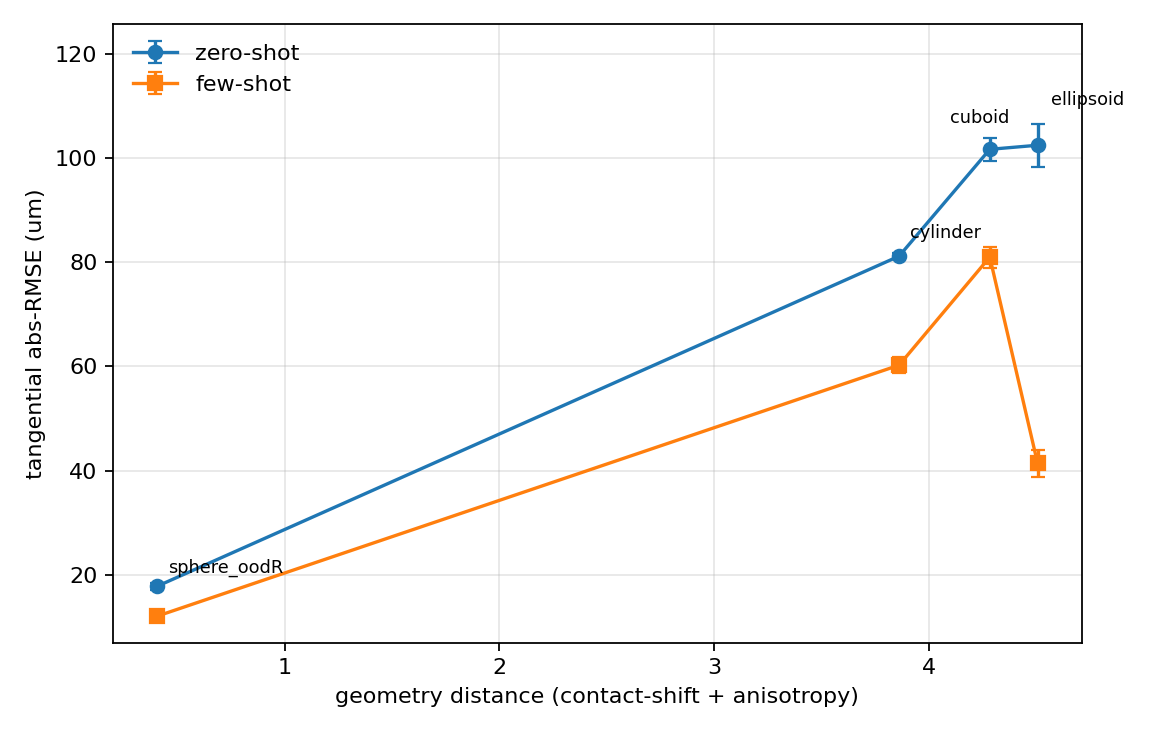
\includegraphics[width=0.92\columnwidth]{figs/geometry_ood.png}
\caption{Out-of-distribution geometry transfer of the sphere-trained operator
(mean$\pm$std over three seeds). Zero-shot error rises monotonically with geometry
distance; a $50$-frame few-shot adaptation lowers it on every shape and beats an
equal-budget from-scratch model (not shown, $46$--$191\,\mu$m).}
\label{fig:geomood}
\end{figure}

\subsection{RQ3: Speed}\label{sec:exp-speed}
The operator runs at $\sim$$\opFps$ frames/s ($\sim$$\opLatency$\,ms latency) versus
$\ipcFps$\,frames/s for a single IPC/GIPC solve at the production tolerance---a
$\sim$$\speedup\times$ speedup over IPC (Fig.~\ref{fig:fidspeed}). At that
tolerance the solver is deterministic, so a single solve is the fair reference and
no replicate averaging inflates the denominator (Appendix~\ref{app:conv}).
We are careful here (Sec.~\ref{sec:limits}):
modern batched GPU physics engines achieve higher aggregate \emph{throughput}. The
operator's durable advantage is the \emph{combination} of low single-frame latency,
cheap differentiability, light hardware, and mesh-freedom---not raw fps.

\begin{figure}[t]
\centering
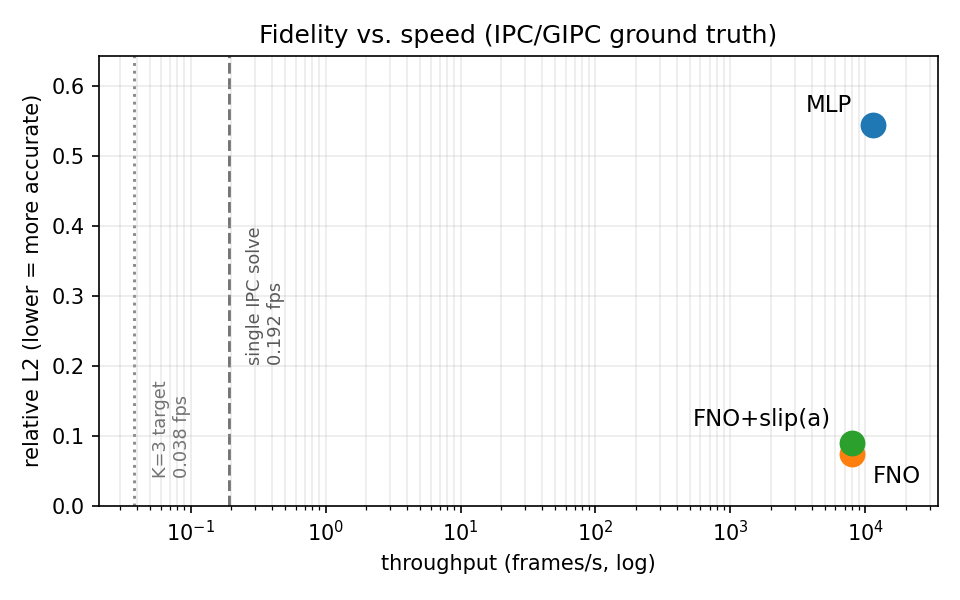
\includegraphics[width=0.92\columnwidth]{figs/fidelity_speed.png}
\caption{Fidelity versus speed. LR-FNO and its multitask variant keep low field
error while moving from second-scale IPC/GIPC solves to sub-millisecond operator
inference. The dashed line is the single-solve IPC reference at the production
tolerance.}
\label{fig:fidspeed}
\end{figure}

\subsection{RQ4: Differentiable control}\label{sec:exp-control}
We train the goal-conditioned servo policy two ways
(Table~\ref{tab:control}, Fig.~\ref{fig:control}). Autograd through the frozen
operator and black-box ES are evaluated on the same IPC dataset. Autograd reaches
a final loss of $\agLoss$ against ES's $\esLoss$, while using
$\mathbf{\agQueries}$ forward evaluations against ES's $\mathbf{\esQueries}$
($\budgetX\times$ smaller evaluation budget) and finishing in
$\mathbf{\agWall}$\,s versus
$\mathbf{\esWall}$\,s ($\wallX\times$ faster). It first reaches the target after
$\agHit$ queries versus $\esHit$ for ES ($\hitX\times$ fewer). Both sit above a
per-instance oracle ($\oracleLoss$), the expected price of a single
amortized network serving
all contexts.

Notably, the gradient pathology of differentiable
simulators~\cite{suh2022diffsim} does \emph{not} appear: autograd gradients are
clean in both stick and slip regimes. This is consistent with the present
single-step quasi-static map, while not establishing the same result for
multi-step contact dynamics.

\begin{table}[t]
\centering
\caption{Goal-conditioned control: autograd through the frozen operator vs.\
gradient-free ES (mean over 3 seeds). Lower loss and far fewer queries.}
\label{tab:control}
\setlength{\tabcolsep}{5pt}
\footnotesize
\begin{tabular}{@{}lccc@{}}
\toprule
 & final loss & fwd queries & wall (s) \\
\midrule
autograd (ours) & $\agLoss$ & $\mathbf{\agQueries}$ & $\mathbf{\agWall}$ \\
ES (pop 32) & $\esLoss$ & $\esQueries$ & $\esWall$ \\
\midrule
per-instance oracle & $\oracleLoss$ & --- & --- \\
\bottomrule
\end{tabular}
\end{table}

\begin{figure}[t]
\centering
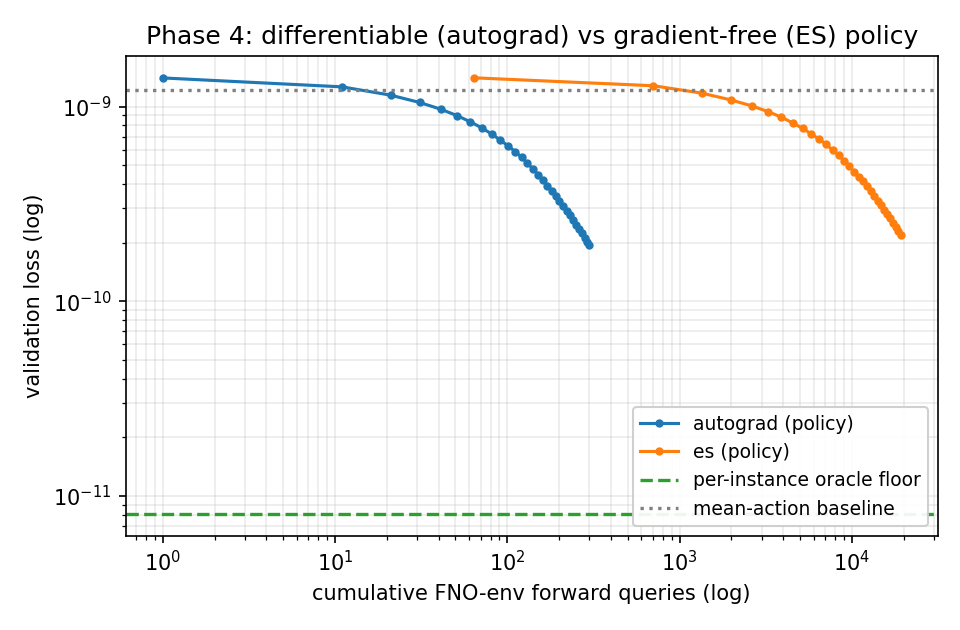
\includegraphics[width=0.92\columnwidth]{figs/policy_servo_curve.png}
\caption{Control convergence vs.\ model queries (log scale). Autograd reaches the
target $\hitX\times$ earlier in query count.}
\label{fig:control}
\end{figure}

\subsection{RQ5: The differentiable sensor and environment}\label{sec:exp-sensor}
The rendered marker flow images in-plane displacement wherever the gel shears:
the cosine between pixel flow and surface in-plane displacement exceeds $\flowCos$
in all four contact regimes---including normal contact, whose small tangential
field is coherent rather than noise-dominated on the corrected ground truth. A
render$\to$track
round trip recovers marker centroids to $\trackStick$\,px in stick,
$\trackPartial$\,px in partial
slip, and $\trackFull$\,px in full slip at $160$\,px resolution
(Fig.~\ref{fig:sensor}). Composing the renderer with the operator, gradient
descent on the rendered \emph{image} recovers applied shear over 20 frames with
$\invMag\%$ mean magnitude error and $\invDir^\circ$ mean direction error; in the
three
shear regimes the direction error is at most $\invDirWorst^\circ$, and both metrics
are hardest in
normal frames, where the applied shear magnitude is near zero and direction
becomes ill-defined.
Finally, wrapping the frozen operator, the sensor, camera noise, and a reward into a
single differentiable environment, the Sec.~\ref{sec:exp-control} policy closes
$\rewardClosed\%$ of the random-to-oracle reward gap. Autograd gradients flow to the
action through the full image pipeline. A finite-difference diagnostic on the
current noisy image-reward environment has $\fdErr\%$ relative error---within the
$5\%$ tolerance---but we still use it only as a gradient-flow sanity check, not as
formal gradient verification or evidence for multi-step contact dynamics.

\begin{figure}[t]
\centering
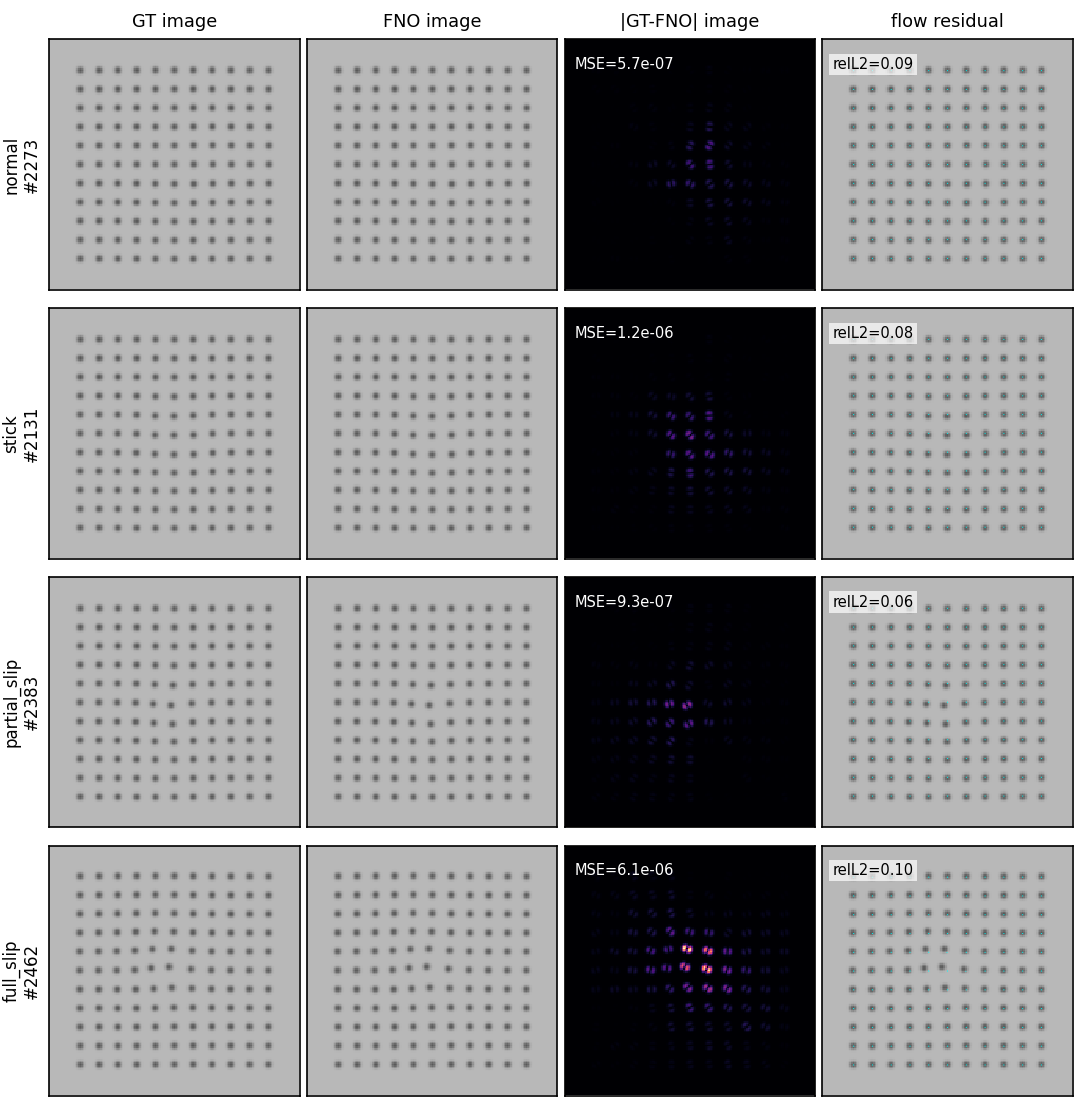
\includegraphics[width=0.95\columnwidth]{figs/sensor_gt_vs_fno.png}
\caption{Rendered marker-dot tactile images across contact modes. Columns show
IPC/GIPC ground truth, LR-FNO prediction, image residual, and residual marker flow.
The differentiable renderer turns the predicted field into a sensor image without
re-solving contact.}
\label{fig:sensor}
\end{figure}

\subsection{Do the conclusions depend on the ground truth?}\label{sec:exp-gtinvariance}
Every result above is measured against a \emph{simulated} target that carries its
own discretisation error (Appendix~\ref{app:conv}). A reader is entitled to ask
whether the comparison survives a better simulator. We test this directly rather
than argue it. We regenerate the entire dataset at a substantially finer
discretisation---gel mesh $24\!\to\!32$ elements per side with $24$ through-thickness
layers, indenter subdivision $2\!\to\!4$ with the barrier width refined in step,
time step halved, Newton tolerance tightened by $30\times$---which moves the target
fields by $24$--$30\%$ in shape, an order of magnitude larger than the surrogate's
own test error. We then retrain every model from scratch on the new targets.

\todo{Run the A/B once the v2 sweep finishes, and report here: (a) the bake-off
table on v2, (b) whether the ranking is preserved, (c) how each margin moves. State
plainly which claims are ground-truth-invariant and which are not. The
\emph{expected} pattern, which must be confirmed, not assumed: margins \emph{between
learned models} are common-mode and should be stable, because all of them are fit on
identical targets; margins against the \emph{analytic} baselines are not
common-mode---those models are fixed physics scored against a moving target---and
may shift. If the ranking does \emph{not} survive, say so and revise the claims.}

Two classes of claim must be distinguished, and only the first is protected by this
design. Margins \emph{among learned models} are common-mode: every model is fit on
the same targets, so a systematic error in those targets largely cancels in the
comparison, and the ranking is a statement about the architectures. Margins against
the \emph{analytic} baselines are not: those are fixed closed-form physics scored
against a target that moves when the solver is refined. We therefore report the
former as the architectural result and the latter with the ground truth it was
measured on named explicitly.

\section{Limitations and Honest Scope}\label{sec:limits}
We state the boundaries plainly, since they shape the contribution.
\textbf{(1) Fidelity is to a solver, not to a sensor.} Our targets come from an IPC
contact solver, and we report that solver's own residual discretisation error rather
than assuming it away (Appendix~\ref{app:conv}): we do \emph{not} claim a converged
ground truth, and once the surrogate's error falls below the solver's, its $\relL$
measures distance to a \emph{particular solver configuration}, not to physical
reality. The two errors are reported separately and must not be added or netted.
What we do establish is that the architectural conclusions are insensitive to a
ground-truth perturbation far larger than the residual (Sec.~\ref{sec:exp-gtinvariance}).
The missing anchor is external, not numerical: the simulated fields model neither
sensor noise nor calibration drift, and no amount of mesh refinement supplies that.
Validation against a physical marker-gel sensor is the necessary next step and is
the honest boundary of the present claims.
\textbf{(2) Single-step quasi-static control.} The environment is a contextual
one-step map rather than multi-step dynamics; temporal contact, hysteresis, and
closed-loop stability require a temporal model and separate evaluation.
\textbf{(3) Sphere-centric geometry.} Training centres on spherical indenters.
We characterise out-of-distribution transfer to six non-spherical shapes
(Sec.~\ref{sec:exp-gen})---error degrades monotonically with geometry distance and
recovers with $50$-frame few-shot adaptation---but zero-shot accuracy on
far-from-sphere objects is not competitive, and a multi-primitive foundation model
for arbitrary-object deployment remains future work. Finally, speed is not claimed as a durable raw-throughput advantage over
modern batched GPU physics; the practical advantage is low latency,
differentiability, and light deployment.

\section{Conclusion}\label{sec:conclusion}
We presented a locally-refined Fourier neural-operator surrogate for vision-based
tactile sensing that is faithful to an IPC contact solver, differentiable, and
hardware-light. The field-to-field framing
exploits the non-locality of elastic contact and beats classical, analytic, and
dense learned tactile models on frictional-contact physics; its differentiability
buys an order-of-magnitude
gain in control sample efficiency; and a torch renderer provides an
autograd-connected image-space loop around the frozen operator. We also audited the
ground truth these claims rest on---something the operator-learning literature
routinely omits---and showed the architectural conclusions survive re-deriving it
at a far finer discretisation. We were explicit about the remaining scope: fidelity
is to a solver rather than to a sensor, the environment is quasi-static, and the
geometry is sphere-centric. The natural next step follows from the boundary we
named: close the sim-to-real loop on a physical marker-gel
sensor, fine-tuning the operator on real measurements so that reality corrects both
discretisation and model error at once.

\appendices
\section{Ground-Truth Convergence Study}\label{app:conv}

We audited the ground truth on three pilot frames spanning the contact modes
(full-slip, stick, partial-slip). All errors are relative $L_2$ on the tangential
surface field; \emph{shape} error is measured after removing the best-fit
amplitude, isolating error that no rescaling can absorb. The reference is the
finest configuration we could afford (gel $48\times48\times24$, indenter
subdivision~4, $\hat d = 2.5\times10^{-5}$\,m).

\textbf{The barrier and the indenter mesh are one knob.} The indenter is a
polyhedron, not a sphere; its geometric error is the facet sagitta
$s \approx e^2/(8R)$ ($s = 5.3\times10^{-5}$, $3.4\times10^{-6}$,
$8.4\times10^{-7}$\,m at subdivision 2, 4, 5 for $R=4.7$\,mm). A barrier thinner
than $s$ resolves the facets rather than the contact, so $\hat d$ and the
subdivision must be refined together. Holding $\hat d / s \approx 7.5$, successive
refinements contract at first order on \emph{all three} modes:
$\{33.5, 26.0, 14.3\}\% \to \{6.6, 6.9, 3.7\}\%$, a ratio of $\approx 0.25$ per
$4\times$ refinement. Refining either knob alone instead produces non-monotone
curves --- an artefact of the two error sources exchanging dominance, not a
property of the solver.

\textbf{Three axes, three signatures.} The contact axis ($\hat d$ with
subdivision) is amplitude-dominated; the gel mesh is shape-dominated
(successive differences $\{10.6, 6.6, 7.5\}\% \to \{5.8, 5.4, 4.9\}\% \to
\{2.7, 4.2, 2.9\}\%$ for $24\!\to\!32\!\to\!40\!\to\!48$); and the time step is
amplitude-dominated and concentrated on partial slip
($\Delta t: 10 \to 5$\,ms changes the field by $\{2.4, 4.0, 13.3\}\%$).
The friction regularisation $\varepsilon_v$ contributes $<2\%$, and the contact
resistance is \emph{not} a refinement parameter (raising it to $10^{11}$ perturbs
the full-slip field by $31\%$).

\textbf{Determinism.} Repeated solves of an identical command differ by $22.6\%$
on a full-slip frame at a loose Newton tolerance ($3\times10^{-4}$) but by only
$0.03$--$0.32\%$ at $10^{-5}$. Run-to-run spread is therefore a property of the
tolerance, not of the GPU, and no replicate averaging is needed at the tolerance
we use.

\textbf{Residual, and what we do \emph{not} claim.} It is tempting to quote the
distance from the production configuration to the finest run we could afford and
call it the error. That number would be misleading: the reference is itself not
converged, and on the time axis it is \emph{coarser} than production, so the
comparison is not even a bound. We therefore follow the standard practice for
solutions without an exact reference and estimate the residual from the observed
convergence order together with the last refinement step. The contact and time axes
contribute a few percent each; the gel-mesh axis is the dominant and
slowest-contracting term, and closing it on every contact mode would cost roughly
an order of magnitude more compute than the dataset itself.

\textbf{We therefore make no claim of a converged ground truth}, and we do not ask
the reader to accept that the residual is negligible. What we do instead is bound
its \emph{consequence}: Sec.~\ref{sec:exp-gtinvariance} retrains every model on
both the pre-refinement ground truth---which this study shows is $24$--$30\%$ off
in field shape, an order of magnitude above the surrogate's own error---and the
refined one, and reports whether the architectural ranking and margins move. A
conclusion that survives a ground-truth perturbation that large does not depend on
the remaining few percent.

\textbf{The anchor we lack.} Convergence establishes only that we solve the
equations we wrote down; it says nothing about whether those equations describe a
real gel. The gold standard in this field is comparison against a physical sensor
(as in the calibration-based simulators we benchmark), and we do not have it. That,
not mesh resolution, is the boundary of our physical claims (Sec.~\ref{sec:limits}).

\section*{Acknowledgment}
We thank the maintainers of the open-source projects this work builds on---in
particular libuipc/GIPC~\cite{huang2024gipc}, the TacEx tactile-simulation
stack~\cite{nguyen2024tacex}, NVIDIA Isaac Sim, and PyTorch.
\todo{funding / grant numbers / hardware support (add after de-anonymisation).}

\bibliographystyle{IEEEtran}
\bibliography{references}

\end{document}
